\chapter{Meaningful Learning}

Meaningful learning refers to the concept that the learned knowledge (lets say a fact) is fully understood by the individual and that the individual knows how that specific fact relates to other stored facts (stored in your brain that is). For understanding this concept, it is good to contrast \textbf{meaningful learning} with the much less desirable, \textbf{rote learning}.

Rote learning is where you memorize something without full understanding and you don't know how the new information relates to your other stored knowledge. For our example, lets say we learn 5 facts in a math course during a full semester by rote learning. This can be illustrated by the figure below. The 5 facts (labeled 1-5) are stored in memory as separate items although in real life they are related to each other. When the student rote learned these facts, the brain stored them as distinct, unrelated knowledge that can only be recalled individually (one fact at a time). When this student recalls one fact the other 4 facts are not recalled (or activated) at that moment. In other words, thinking about fact \#5 does not lead the student to think about facts \#1-4. Contrast that to the below discussion on recall after meaningful learning.

\begin{figure}
	\centering
	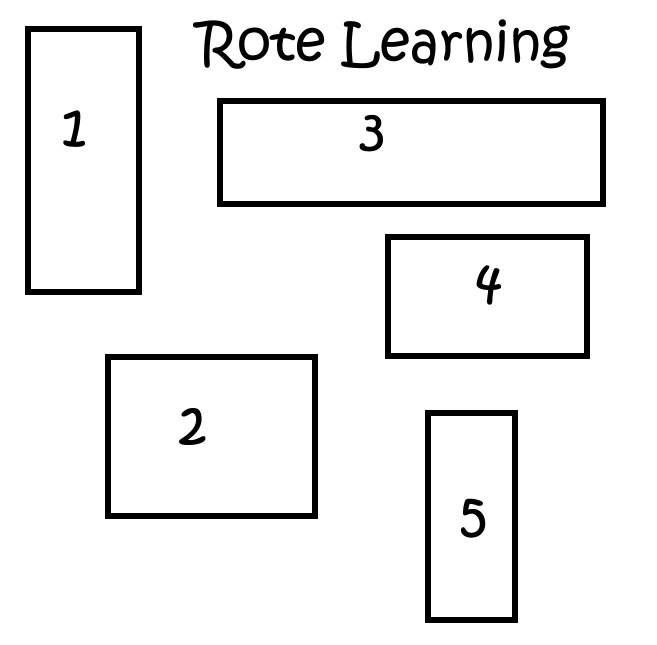
\includegraphics[width=0.55\linewidth]{./images/mean1}
	\caption{Rote Learning}
	\label{fig:mean1}
\end{figure}

When meaningful learning occurs (using our example of 5 math facts) the facts are stored in a relational manner (see figure below). That is, the brain stores them together because they are related to each other. Now, when one fact is recalled, the other facts are also recalled at that moment (or shortly thereafter). In other words, recalling fact \#5 activates the memory for facts \#2 and \#4, and this in turn leads to recalling facts \#1 and \#3. This phenomenon is called the spread of activation. This is the gist of meaningful learning. Problem-solving for this student would be easier than for the student who rote learned the same 5 facts.  Which one of these students would you like to hire for your company? Some suggestions on how to ensure meaningful learning appear below the figure. 

\begin{figure}
	\centering
	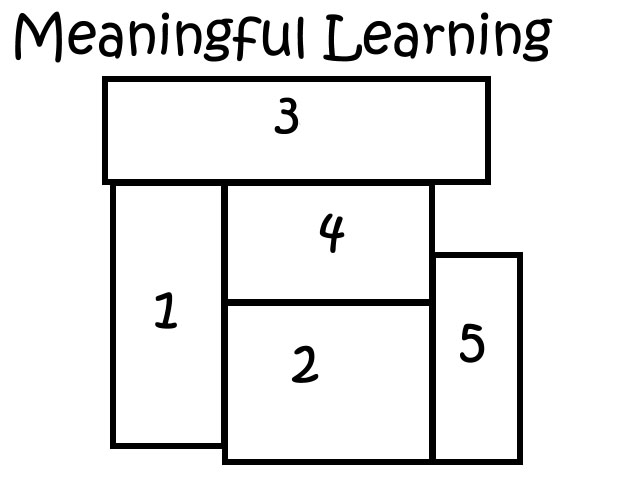
\includegraphics[width=0.55\linewidth]{./images/mean2}
	\caption{Meaningful Learning}
	\label{fig:mean2}
\end{figure}

\section{Suggestions}

\begin{itemize}
	\item Make sure what you learn is in your proximal zone.
	\item If in doubt, ask the instructor how some new knowledge is related to other course material.
	\item Have a study partner ask you questions that require recall of related material.
	\item Make a figure that illustrates what you should know about a specific topic and its related material.
\end{itemize}